\section{\method{} with a critic: pathwise RL}
\label{sec:method}
\method{}-GRPO differentiates the density of the chain; the two variants of this section differentiate the chain itself. The reward is not differentiable, since $r$ depends on $s_{K-1}$ through an $\arg\max$ and a program, but the value~(\ref{eq:value}) of an earlier state is. Both variants learn a differentiable estimate $V_\phi$ of it, a critic trained together with the policy, and ascend it through one transition of the chain. They differ in the critic: one value per state in \method{}-Scalar, one per state and position in \method{}-2D.

\begin{figure}[t]
\centering
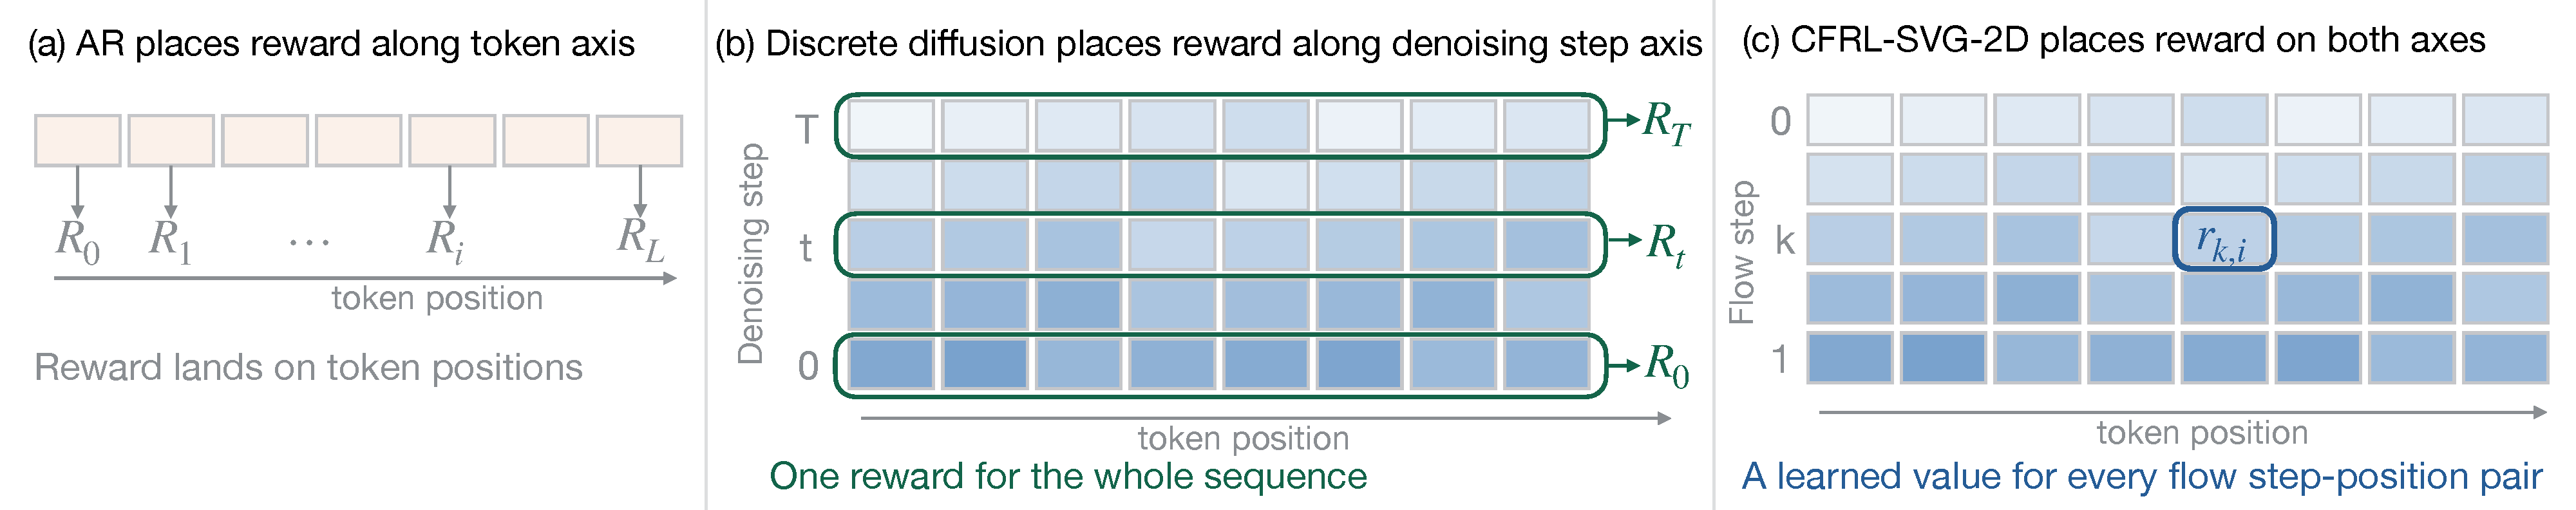
\includegraphics[width=0.9\linewidth]{figures/flow-rl-figure1.pdf}
\caption{Where the reward lands: (a) along the token axis in an AR model; (b) along the denoising-step axis in RL for discrete diffusion, one value for the whole sequence; (c) in \method{}-2D on both, a value $R_{k,i}$ for every flow step $k$ and position $i$, pooled into the actor's objective $V_\phi$ and trained on the outcome $r$ of the policy's own rollouts.}
\label{fig:mechanism}
\end{figure}

\subsection{The pathwise update}
\label{sec:pathwise}
Fix a prompt and give transition $k$, the denoiser call at $s_{k-1}$ followed by the re-noise, its own copy $\theta_k$ of the parameters, tied to $\theta$ after differentiation, so that $\nabla_\theta J=\sum_{k=2}^{K-1}\partial J/\partial\theta_k$. The objective depends on $\theta_k$ only through the state $s_k=(y_k,\hat x_{k-1})$, both components of which are outputs of that call: $y_k=\alpha_kD_{\theta_k}(s_{k-1})+\sigma_k\varepsilon_k$ with $D_\theta(s_{k-1})=y_{k-1}+\lambda_{k-1}(\hat x_{k-1}-y_{k-1})$. The downstream value $V_k$ does not depend on $\theta_k$ and is a Gaussian smoothing of a bounded function, so the expectation is differentiated inside with the noise held fixed (Appendix~\ref{app:pw_derivation}):
\begin{equation}
\frac{\partial J}{\partial\theta_k}=\mathbb E\big[\nabla_{\theta_k}V_k(s_k)\big],\qquad \nabla_{\theta_k}V_k(s_k)=\Big[\alpha_k\lambda_{k-1}\nabla_{y}V_k(s_k)+\nabla_{\hat x}V_k(s_k)\Big]\frac{\partial\hat x_{k-1}}{\partial\theta_k},
\label{eq:pw_exact}
\end{equation}\eqalias{eq:chainrule}
the first term through the re-noised state, the second through the estimate that the next call reads. By Gaussian integration by parts the first term has the same expectation as the $k$-th summand of the score-function form. The two differ in what multiplies the denoiser's Jacobian at coordinate $(k,i)$: the factor $V_k\,\varepsilon_{k,i}/\sigma_k$, of variance $\approx\mathbb E[V_k^2]/\sigma_k^2$ whether or not the coordinate affects the outcome, against the derivative $\partial V_k/\partial y_{k,i}$, which vanishes on every coordinate the value does not depend on.

\paragraph{The estimator.}
The critic $V_\phi$ that replaces $V_k$ is trained in logit units (\S\ref{sec:critic}). With an exact critic the sample gradient is $\nabla\mathrm{logit}\,V_k=\nabla V_k/[V_k(1-V_k)]$, the sample's term of~(\ref{eq:pw_exact}) scaled by a positive weight, so the update ascends the expected log-odds of success. One transition is drawn from a window $\mathcal W=\{k_{\rm lo},\dots,k_{\rm hi}\}$ in the middle of the chain:
\begin{equation}
\tilde J_k=\mathbb E[\mathrm{logit}\,V_k(s_k)],\quad \hat g_{\rm PW}=\nabla_\theta V_\phi(s_k),\ k\sim\mathcal U(\mathcal W),\quad \text{bias: }\mathbb E[\nabla_\theta(V_\phi{-}\mathrm{logit}\,V_k)(s_k)].
\label{eq:pw}
\end{equation}\eqalias{eq:logodds}\eqalias{eq:biasm}
The chain is rolled to $s_{k-1}$ without gradients and the call at $s_{k-1}$ is taken with gradients, so the memory does not depend on $K$: the rest of the chain is carried by the value in expectation, not by back-propagation. Log-odds are the scale on which a critic trained by cross-entropy is calibrated, and their weight keeps the signal alive where the outcome is nearly decided. The window leaves out the first steps, where the state is noise and the value flat, and the last, where the state is committed. There is no baseline, advantage or trust region; a baseline is constant in the noise and contributes nothing to a pathwise gradient. What the update does carry is the bias of~(\ref{eq:biasm}), which vanishes when the critic's slope matches that of the log-odds on the states the current policy visits; the critic is designed and trained for that condition.

\subsection{The critic: one value per state, or per state and position}
\label{sec:critic}\label{sec:jpc_scalar}\label{sec:jpc_2d}
The critic reads what the value is a function of, the state $s_k=(y_k,\hat x_{k-1})$ and the time $\tilde t_k$. The estimate $\hat x_{k-1}$ is the informative part, the denoiser's reading of what the noisy state will decode to, and the denoiser is the network that can compute it. The critic therefore reuses it: a copy $\hat X_\phi$ of the denoiser, evaluated without guidance, gives per-position features, and a three-layer MLP head $h_\phi$ turns them into a value in one of two orders,
\begin{align}
f_i(s_k)&=\hat X_\phi(y_k,\tilde t_k;\hat x_{k-1})_i\in\mathbb R^d, &\text{\method{}-Scalar:}\quad V_\phi(s_k)&=h_\phi\Big(\tfrac1{|\mathcal G|}\textstyle\sum_{i\in\mathcal G}f_i(s_k),\,\tilde t_k\Big),
\label{eq:critic1d}\\
R_{k,i}&=h_\phi\big(f_i(s_k),\tilde t_k\big), &\text{\method{}-2D:}\quad V_\phi(s_k)&=\tfrac1{|\mathcal G|}\textstyle\sum_{i\in\mathcal G}R_{k,i}.
\label{eq:critic2d}
\end{align}\eqaliasprev{eq:feat}
A flow model generates all positions at once and refines them over $K$ steps, so credit has two axes, \emph{when} along the flow and \emph{where} along the sequence (Figure~\ref{fig:mechanism}). RL for diffusion and flow models indexes it by the step and treats the whole state as one action \citep{liu2025flowgrpo,xue2025dancegrpo}, as \method{}-GRPO and \method{}-Scalar do; \method{}-2D indexes the value by both. The actor ascends the pooled value through~(\ref{eq:pw}) in both, and only the order of head and mean differs. It decides what each position is asked to change. The actor's signal at position $i$ is $\sum_{j}(\partial V_\phi/\partial f_j)(\partial f_j/\partial y_{k,i})$, where
\begin{equation}
\text{head after the mean: }\ \frac{\partial V_\phi}{\partial f_j}=\frac{\nabla h_\phi(\bar f)}{|\mathcal G|}\ \ \forall j,\qquad \text{head before the mean: }\ \frac{\partial V_\phi}{\partial f_j}=\frac{\nabla h_\phi(f_j)}{|\mathcal G|},
\label{eq:headgrad}
\end{equation}
with $\bar f$ the mean feature. Either every position is pushed along one direction of feature space, the head's slope at the mean, or each along the head's slope at its own reading, the change that would raise its own estimate of success. For one policy and one batch the two updates are close, since both heads read the same features and fit the same outcome; the difference is made over training, where the policy moves and the head is refit. A head on the mean can moreover depend on the positions only affinely, through the bottleneck $\bar f$ (Proposition~\ref{prop:additive}).

\paragraph{Supervision without token labels.}
Both critics are trained on states of rollouts, each labelled with its rollout's outcome $r$,
\begin{equation}
\mathcal L_{\rm 2D}(\phi)=\tfrac12\,\mathrm{BCE}\big(\mathrm{sig}(V_\phi(s_k)),r\big)+\tfrac12\,\frac1{|\mathcal G|}\sum_{i\in\mathcal G}\mathrm{BCE}\big(\mathrm{sig}(R_{k,i}),r\big),
\label{eq:critic2d_loss}
\end{equation}\eqalias{eq:bce}
the scalar critic with the first term only. The first term is minimised by $\mathrm{sig}(V_\phi(s))=V_k(s)$: the critic is fitted to the log-odds that~(\ref{eq:pw}) ascends. The second makes every reading a calibrated log-odds on its own; without it the field is constrained only through its mean. A head on the mean is one function of one vector, which the actor can raise by moving that vector wherever the head reads success, whereas a rise of the pooled field has to be carried by $|\mathcal G|$ calibrated readings. $R_{k,i}$ is not a verifier of token $i$: every reading predicts the outcome of the whole response, and within a failed response the readings barely tell wrong positions from right ones (Appendix~\ref{app:critic_maps}). What the field buys is its behaviour under joint training (\S\ref{sec:exp_2d}), not localisation.

\subsection{Training the critic with the policy}
\label{sec:joint}
The bias of~(\ref{eq:biasm}) has two moving targets. As $\theta$ changes, so do the states the policy visits, and so does $V_k$ itself, which depends on the transitions after step $k$: a critic fitted to an earlier policy is wrong even on a state it has seen, and the actor, which ascends $V_\phi$ wherever its slope is positive, exploits it. The critic is pre-trained on rollouts of the initial policy, copy and head together, and Algorithm~\ref{alg:jpc} then refits it after every actor step: the head only, on a replay buffer of the states that fresh rollouts reach at the top of the window, where the state determines the outcome best. The copy stays frozen, since refitting it would cost a fine-tuning step per actor step and move the actor's objective between steps. If the critic's AUC on the newest buffer states falls below a floor, the head takes extra steps before the actor moves again. The bias is paid at every actor step in proportion to the step, so the actor's step size decays, and both networks are trained under the sampler that will be deployed, a different sampler being a different chain with different values (Appendix~\ref{app:joint_details}).

\begin{algorithm}[t]
\caption{\method{} with a critic (\method{}-Scalar: critic~(\ref{eq:critic1d}); \method{}-2D: critic~(\ref{eq:critic2d}))}
\label{alg:jpc}
\small
\begin{algorithmic}[1]
\REQUIRE SFT policy $\hat X_\theta$; pre-trained critic $V_\phi$ (frozen copy $\hat X_\phi$, trainable head $h_\phi$); verifier $r$; sampler $(\gamma,K)$; window $\mathcal W=\{k_{\rm lo},\dots,k_{\rm hi}\}$; replay buffer $\mathcal B$ of capacity $N_{\mathcal B}$
\FOR{iteration $=1,\dots,T$}
  \STATE \textbf{Actor.} For $B$ prompts and one $k\sim\mathcal U(\mathcal W)$: roll out to $s_{k-1}$ without gradients, take the denoiser call at $s_{k-1}$ with gradients to form $s_k$, and set $\theta\leftarrow\theta+\eta_\theta\,\mathrm{AdamW}\big(\nabla_\theta\frac1B\sum_{b}V_\phi(s_k^{(b)})\big)$ \hfill ($\phi$ fixed; eq.~\ref{eq:pw})
  \STATE \textbf{Buffer.} Roll out $B$ fresh prompts to the end, decode, verify; push each $(s_{k_{\rm hi}},r)$ into $\mathcal B$
  \STATE \textbf{Critic.} $m_{\rm c}$ head steps $\phi\leftarrow\phi-\eta_\phi\,\mathrm{AdamW}(\nabla_\phi\mathcal L_{\rm 2D})$ on minibatches of $\mathcal B$; every $n_q$ iterations, $m'_{\rm c}$ more if the AUC of $V_\phi$ on the newest $N_q$ states is below $a_0$ \hfill (eq.~\ref{eq:critic2d_loss})
\ENDFOR
\end{algorithmic}
\end{algorithm}

\paragraph{Amortising the policy into the model.}
\label{sec:loop}
The gain of the pathwise variants belongs to the chain they were trained under. An optional last step moves it into the model's supervised objective, which trains the denoiser at every time $t$: a round draws responses from the policy on a pool of unlabelled prompts, keeps the verified, distinct ones, and fine-tunes the model on them with ELF's own loss (Algorithm~\ref{alg:loop}, Appendix~\ref{app:loop}). This is rejection-sampling fine-tuning \citep{yuan2023rft,singh2023restem,zelikman2022star} with the RL policy as the sampler, the M-step of an EM view of~(\ref{eq:objective}) whose lower bound on the reward is tight at the current model (Proposition~\ref{prop:em}). A round teaches nothing on a prompt without an accepted response, so its reach is the pool's coverage. There the 2D critic serves a second time: read through its most pessimistic position, $\min_{i}\mathrm{sig}(R_{k,i})$, it prunes parallel chains and nudges the state along its gradient before the verifier can act, so that pools can be drawn with a cheap chain.
